\chapter{The Z-Way HA User Manual}
\label{vdev}

The intention of the virtual Device API (vDev) is to further simplify the use of Z-Way
by AJAX based User interface implementations. The implementation is based on the
Javascript module concept  and the use of the vDev API is demonstrated with the 
demo UI 'z-way-ha'. You can access the User Interface 'z-way-ha' using the URL

\paragraph{http://YOURIP:8083/z-way-ha}
\paragraph{}

The following sections describes the 'Z-Way-HA' from the users point of view  

The Z-Way-HA User Interface is a AJAX based user interface available for web browsers. At 
the moment it supports Google Chrome, Firefox and Apple Safari only but no Microsoft Internet
Explorer.

The functions of the Z-Way-HA UI are:

\begin{itemize}
\item show all device functions of the Z-Way based Smart Home systems as widgets
\item allow to activate and manage automation modules that make use of the widgets
and may generate new widgets
\end{itemize}

The User Interface offers four function groups:

\begin{itemize}
\item \textbf{Dashboard}: Important widgets are shown in the dashboard. The section 'widgets'
in the 'Preferences' allow to define what widget is shown in the Dashboard.
\item \textbf{Widgets}: The widget section allows to access all widgets of the Home 
Automation System. They are grouped by 'Rooms', 'Type', and 'Tags' The 'Preferences'
allow to manage rooms, types and widgets and to assign certain widgets to these groups.
\item \textbf{Notifications}: Clocking om the notifications button opens a dialog showing all 
notification generated by the system and the modules. Notifications will stay in this list
until these are individually confirmed.
\item \textbf{Preferences}: The preferences tab opens a dialog with different setup options.
\begin{itemize}
\item \textbf{General}:  This allows to setup and manage profiles
\item \textbf{Rooms}:  This allows to setup and manage rooms
\item \textbf{Widgets}:  This allows managing widgets
\item \textbf{Automation}:  This allow managing the modules of the Javascript based 
automation engine
\end{itemize}
\end{itemize}

\subsection{Widgets}

The widget section allows managing all widgets that are automatically created from the 
device included into the Z-Wave or Third party Wireless Control System plus the widgets
generated from Automation Modules.\footnote{Technically also te widgets from the wireless 
control systems are generated by modules but this happens automatically when they registered
resp. included in the wireless system.}

A widget does not necessarily represent a physical device but a function of a device.
This means that one single device can create multiple widgets.
For Z-Wave devices every function (switch, battery, sensor value) and every channel in 
a multichannel environment generated a widget. The widget is not technology dependent but 
the initial name and the unique id of the generated widget is referring to the attributes 
of the physical  device. The pattern for the id is

\paragraph{ZWayVDev\_[Node ID]:[Instance ID]:[Command Class ID]:[Scale ID]}

\paragraph{}

The Node ID referred to the node ID of the physical device corresponding to thie widget, 
the instance is the instance or zero in case there are no multiple instances.
The command class ID refers to the command class generated the function of the widget.
Some command classes offer multiple sensor values differentiated by their scale id (e.g. 
Celsius or Fahrenheit). For command classes without multiple scales (e.g. battery value) 
this value is always zero.

The line below the main menu offers three options grouping the widgets:

\begin{itemize}
\item \textbf{by Room}:  The Ui can define rooms and in the room definitions widgets
can be assigned to rooms. Each widget can be assigned only to one room. The line below shows
all rooms currently defined. Clicking on the room shows all widgets assigned to this room. 
To manage rooms please refer to the section Preferences.
\item \textbf{by Type}:  All Widgets belong to one specific type. At the moment the following
types are defined and supported by the Z-Way-HA UI:
\begin{itemize}
\item \textbf{sensorBinary}: A binary sensor, only showing on or off
\item \textbf{sensorMultilevel}: The type, the value and the scale of the sensor are shown
\item \textbf{switchBinary}: The device can be switched on and off
\item \textbf{switchMultilevel}: The device can be switched on and off plus set to any
percentage level between 0 \% and 100 \%.
\item \textbf{switchRGBW}: This device allows setting RGB colors
\item \textbf{switchControl}:
\item \textbf{toggleButton}: The device can only be toggled between on and off.
\item \textbf{thermostat}: The thermostat shows the setpoint temperature plus a drop 
down list of thermostat modes if available
\item \textbf{battery}: The battery widget just shows the percentage of charging capacity left
\item \textbf{camera}: A camera will show the image and can be operated
\item \textbf{fan}: A fan can be turned on and off
\end{itemize}
The line below shows
all types where devices exist. Device types can not be managed on the UI but will be shown
automatically when new widgets are generated.
\item \textbf{By Tag}:  The system allows to generate user defined tags and assign 
these tags to defines. The only predefined tag is the 'dashboard'. This tag is used to 
select all widgets that are shown in the dashboard.
The line below shows all tags currently defined. Clicking on the tags shows all 
widgets assigned where this tag is assigned to. Tags can be freely defined when managing
a certain widget.
\end{itemize}

\subsection{Notifications}

Left beside the Notification button the number of notifications are shown. Clicking on 
the String 'Notification' opens a dialog box with the notification string. Notifications
are generated by the system (error message) or by application modules.
'Hide' deletes the message.

\subsection{Preferences}

Clicking on 'Preferences' opens a dialog with four sub menus as shown in Figure 
\ref{ha_prefs}. One the upper 
side there is a 'X' to close the dialog. Once a sub menu is opened on the 
upper left side the '<' returns to the sub menu overview.

\begin{figure} 
\begin{center}
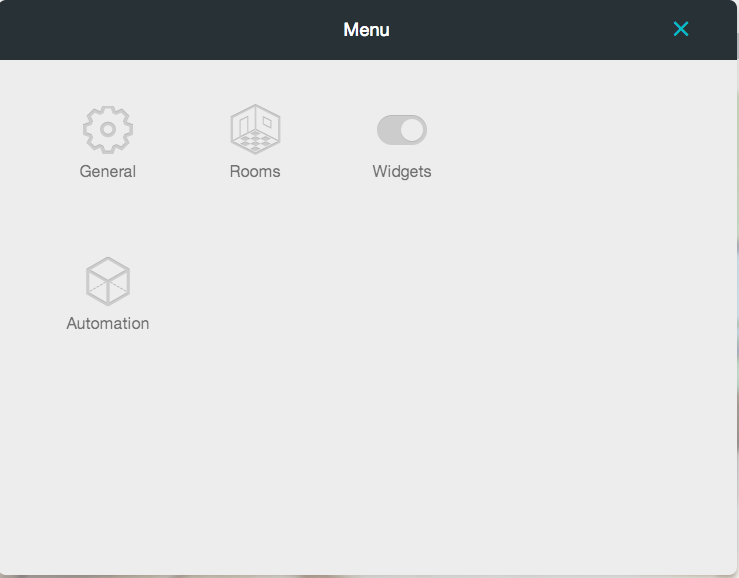
\includegraphics[width=0.8\textwidth]{pics/ha_preferences.png}
\caption{Preferences Submenu}
\label{ha_prefs}
\end{center} 
\end{figure}


\subsubsection{General}

The dialog shows different profiles. At the moment there are no further options 
and actions available except naming the profiles and giving a Name.

On the lower left corner there is a '-' and a '+'. Clicking on the '+' adds a new
profile, '-' deletes the profile highlighted on the left hand side. A filter can 
be applied to find certain profiles.

On factory default only the 'default' profile is available.

\subsubsection{Rooms}

The dialog 'Rooms' offers four submenus.

On the lower left corner there is a '-' and a '+'. Clicking on the '+' adds a new
room, '-' deletes the room highlighted on the left hand side. A filter can 
be applied to find certain rooms.

\paragraph{General}

Clicking on the 'Edit'-Button allows editing the Room setup.

The name can be chosen by the user. Clicking on the icon image opens a file chooser 
dialog to pick a new icon. Clicking on the device button opens a new dialog where 
devices can be assigned to this room. The left hand side shows the device available (not 
assigned ot any room). Picking the device is done by 'drag and drop'.
Devices on the right hand side are assigned to the room.

\paragraph{Temperature Preference}

This dialog is not used at the moment.

\paragraph{Auto Mode}

This dialog is not used at the moment.

\paragraph{Devices}

This is a short cut to the device assignment dialog also accessible in the 'General'
sub menu.

\subsubsection{Widgets}

The widgets menu allows managing the widgets generated by the 
Home Automation system. All widget are listed with their names on the left hand side.
A filter can be applied to find certain widgets.

The name of the widget is auto-generated by the system but can be changed. The id of the 
widget is unique and shown below the name entry.
The device type is shown.

The tag section allows to add new tags defined by the user. 
Defined tags are listed and can be deleted clicking on the 'x' symbol.

A checkbox defined if the widget is shown on the dash board.

\subsection{Dashboard}

The dashboard shows all widgets selected as 'in dashboardÄ in the widget 
dialog of the Preferences section.

\subsubsection{Automation}

This section


